%macbook 
\setcounter{paragraph}{0}
\PhanI
\loai{Khoảng cách giữa hai cực đại hoặc hai cực tiểu liên tiếp trên đoạn hai nguồn}
\begin{ex}%KNTT
\immini[thm]{Trong thí nghiệm như hình vẽ, hai nguồn sóng tại $S_1$ và $S_2$ có tốc độ truyền sóng trên mặt nước là 50 cm/s, cần rung có tần số 40 Hz. Khoảng cách giữa hai điểm cực đại giao thoa cạnh nhau trên đoạn thẳng $S_1S_2$ là
\motcot
{0,982 cm}
{0,564 cm}
{0,234 cm}
{\True 0,625 cm}
}{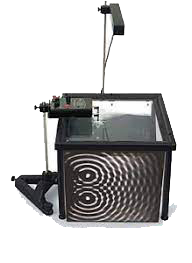
\includegraphics[width=4cm]{Hinh/KN121}}
\loigiai{
\begin{itemize}
\item Khoảng cách giữa hai điểm cực đại giao thoa cạnh nhau trên đoạn thẳng $S_1S_2$ là: $\dfrac{\lambda}{2}=\dfrac{v}{2f}=\dfrac{50}{2.40}=0,625\ cm$.
\end{itemize}
}
\end{ex} \haidong{20}

\begin{ex}%[3P2B5-2][Loai1]
\nguon{MH - 2018} Giao thoa ở mặt nước được tạo bởi hai nguồn sóng kết hợp dao động điều hòa cùng pha theo phương thẳng đứng tại hai vị trí $S_1$ và $S_2$. Sóng truyền trên mặt nước có bước sóng 6 cm. Trên đoạn thẳng $S_1S_2,$ hai điểm gần nhau nhất mà phần tử nước tại đó dao động với biên độ cực đại cách nhau
\choice
{12 cm}
{6 cm}
{\True 3 cm}
{1,5 cm}
\loigiai{
Trên đoạn thẳng nối hai nguồn, hai điểm gần nhau nhất mà phần tử nước tại đó dao động với biên độ cực đại cách nhau 1 khoảng bằng $\dfrac{\lambda}2=3\ cm$.
}

\end{ex} \haidong{20}

\begin{ex}%[3P2-5.2Y][Loai1] 
\nguon{QG - 2018} Trong thí nghiệm giao thoa sóng trên mặt nuớc, hai nguồn kết hợp đặt tại hai điểm A và B dao động cùng pha theo phương thẳng đứng. Sóng truyền trên mặt nước có bước sóng là 4 cm. Trên đoạn thẳng AB, khoảng cách giữa hai cực đại giao thoa liên tiếp là
\choice
{8 cm}
{\True 2 cm}
{1 cm}
{4 cm}
\loigiai{
Trên đoạn thẳng AB, khoảng cách giữa hai cực đại giao thoa liên tiếp là $\dfrac{\lambda}2 =\dfrac{4}2 =2$ cm.
}
\end{ex} \haidong{20}
\loai{Biết khoảng cách giữa hai cực đại hoặc cực tiểu, tìm bước sóng và tốc độ truyền sóng}
\begin{ex}%[3P2B5-2][Loai1] 
\nguon{QG - 2018} Trong thí nghiệm giao thoa sóng ở mặt nước, hai nguồn kết hợp đặt tại hai điểm A và B dao động cùng pha theo phương thẳng đứng. Trên đoạn thẳng AB, khoảng cách giữa hai cực đại giao thoa liên tiếp là 2 cm. Sóng truyền trên mặt nước có bước sóng là
\choice
{1 cm}
{\True 4 cm}
{2 cm}
{8 cm}
\loigiai{
Hai cực đại giao thoa liên tiếp cách nhau $\dfrac{\lambda}{2}$.
}
\end{ex} \haidong{20}

\begin{ex}%[3P2B5-2][Loai1] 
Trong thí nghiệm tạo vân giao thoa sóng trên mặt nước, người ta dùng nguồn dao động có tần số 50 Hz và đo được khoảng cách giữa hai cực đại liên tiếp nằm trên đường nối hai tâm dao động là 2 mm. Tốc độ truyền sóng trên dây là
\choice
{40 cm/s}
{10 cm/s}
{\True 20 cm/s}
{30 cm/s}
\loigiai{
\begin{itemize}
\item Khoảng cách giữa hai cực đại liên tiếp là $\dfrac{\lambda}{2} = 2\ mm\ \Rightarrow \lambda =4\ mm \Rightarrow v = \lambda .f = 50.4 = 200 = 20$ cm/s.
\item 
\end{itemize}
}
\end{ex} \haidong{20}
\loai{M là cực đại, cho số cực đại giữa M và đường trung trực}
\begin{ex}%[3P2K5-2][Loai1]
Trong thí nghiệm giao thoa sóng trên mặt nước, hai nguồn kết hợp dao động cùng pha $O_1$ và $O_2$ cách nhau 20,5 cm dao động với cùng tần số $f=15$ Hz. Tại điểm M cách hai nguồn những khoảng $d_1 =23$ cm và $d_2=26,2$ cm sóng có biên độ cực đại. Biết rằng giữa M và đường trực của $O_1O_2$ còn một đường cực đại giao thoa. Vận tốc truyền sóng trên mặt nước là
\choice
{2,4 m/s}
{16 cm/s}
{48 cm/s}
{\True 24 cm/s}
\loigiai{
\begin{itemize}
\item Tại M sóng có biên độ cực đại nên ta có: $d_1-d_2 = k \lambda$.
\item Hai nguồn dao động cùng pha nên trung trực của hai nguồn là một cực đại giao thoa, giữa M và trung trực có một vân cực đại nên M thuộc vân cực đại $|k|=2$.
\item Như vậy ta có $\lambda = 1,6\ cm \Rightarrow v = 24\ cm /s$.
\end{itemize}
}
\end{ex} \haidong{20}
\begin{ex}
Trong thí nghiệm giao thoa sóng trên mặt nước, hai nguồn $A$, $B$ dao động cùng pha với cùng tần số $12\ Hz$. Tại một điểm $M$ cách các nguồn $A$, $B$ lần lượt là $19\ cm$ và $21\ cm$ thì sóng có biên độ cực đại. Giữa $M$ và đường trung trực của $AB$ có đúng một dãy cực tiểu. Tốc độ truyền sóng trên mặt nước là
\choice
{$24\ m/s$}
{$12\ m/s$}
{\True $24\ cm/s$}
{$12\ cm/s$}
\loigiai{
\begin{itemize}
\item[A] Sai vì đơn vị tính nhầm sang $m/s$.
\item[B] Sai vì nhầm hệ số.
\item[C] Đúng: vì $\Delta d=2\ cm=\lambda$, $v=f\lambda=12\cdot2=24\ cm/s$.
\item[D] Sai vì nhầm tần số hoặc bước sóng.
\end{itemize}
}
\end{ex}
\loai{Xác định 1 điểm thuộc cực đại hai cực tiểu}
\begin{ex}
Trong thí nghiệm về giao thoa sóng, hai nguồn kết hợp $A$, $B$ dao động cùng tần số $10\ Hz$ và cùng pha. Tốc độ truyền sóng trên mặt nước là $30\ cm/s$. Tại một điểm $M$ cách nguồn $A$, $B$ lần lượt $31\ cm$ và $25\ cm$ là vân cực đại hay cực tiểu thứ mấy tính từ đường trung trực của $AB$?
\choice
{Cực tiểu thứ 2}
{\True Cực đại thứ 2}
{Cực tiểu thứ 3}
{Cực đại thứ 3}
\loigiai{ }
\end{ex}
\begin{ex}%[3P2K5-2][Loai1]
Tại hai điểm $S_1,\ S_2$ trên mặt nước đặt hai nguồn kết hợp giống nhau có tần số 50 Hz. Tốc độ truyền sóng trong nước là 25 cm/s. Coi biên độ sóng không đổi khi truyền đi. Hai điểm M, N nằm trên mặt nước với $S_1M = 14,75$ cm, $S_2M = 12,5$ cm và $S_1N = 11$ cm, $S_2N = 14$ cm. Kết luận nào sau đây là đúng?
\choice
{M dao động biên độ cực đại, N dao động biên độ cực tiểu}
{M, N dao động biên độ cực đại}
{\True M dao động biên độ cực tiểu, N dao động biên độ cực đại}
{M, N dao động biên độ cực tiểu}
\loigiai{
\begin{itemize}
\item Điểm M có: $\dfrac{\left| M{S_1{1}}-M{S_1{2}} \right|}{\lambda }=4,5=5-0,5 \Rightarrow$ M thuộc dãy cực tiểu số 5 tính từ đường trung trực đi ra.
\item Điểm N có: $\dfrac{\left| N{S_1{1}}-N{S_1{2}} \right|}{\lambda }=6 \Rightarrow$ N thuộc dãy cực đại số 6 tính từ đường trung trực đi ra.
\item 
\end{itemize}
}
\end{ex} \haidong{20}
\loai{M là cực đại, cho số cực đại giữa M và đường trung trực}
\begin{ex}%[3P2K5-2][Loai1]
Trong thí nghiệm về giao thoa sóng trên mặt nước, hai nguồn kết hợp A, B dao động giống hệt nhau với tần số 16 Hz. Tại điểm M cách nguồn A, B những khoảng $d_1=30$ cm, $d_2=25,5$ cm sóng có biên độ cực đại. Giữa M và đường trung trực của AB có 2 dãy các cực đại khác. Vận tốc truyền sóng trên mặt nước là
\choice
{\True 24 cm/s}
{36 cm/s}
{12 cm/s}
{100 cm/s}
\loigiai{
\begin{itemize}
\item Hai nguồn kết hợp A, B dao động giống hệt nhau $\Rightarrow$ Trung trực AB là vân cực đại đại trung tâm.
\item Giữa M và đường trung trực của AB có 2 dãy các cực đại khác $\Rightarrow$ M thuộc cực đại bậc 3.
\item Ta có $d_1-d_2 = 4,5 = 3.\lambda  = 3.\dfrac{v}{f} \Rightarrow v = \dfrac{4,5.16}{3} = 24\ cm/s$. 
\item 
\item
\end{itemize}
}
\end{ex} \haidong{20}
\loai{Xác định 1 điểm thuộc cực tiểu thứ mấy}
\begin{ex}%[3P2K5-2][Loai1]
Trong thí nghiệm giao thoa trên mặt nước, hai nguồn kết hợp giống nhau dao động với tần số 80 Hz, tốc độ truyền sóng 0,8 m/s. Tính từ đường trung trực của hai nguồn, điểm M cách hai nguồn lần lượt 20,25 cm và 26,75 cm nằm trên
\choice
{đường cực tiểu thứ 6}
{\True đường cực tiểu thứ 7}
{đường cực đại bậc 6}
{đường cực đại bậc 7}
\loigiai{
\begin{itemize}
\item Điểm M có: $\dfrac{\left| M{S_1{1}}-M{S_1{2}} \right|}{\lambda }=6,5=7-0,5 \Rightarrow$ M thuộc dãy cực tiểu số 7 tính từ đường trung trực đi ra.
\end{itemize}
}
\end{ex} \haidong{20}
\loai{Cho số cực đại hoặc cực tiểu trên đoạn hai nguồn, tìm các đại lượng}
\begin{ex}%[3P2K5-2][Loai1]
Trên mặt chất lỏng có hai nguồn sóng kết hợp A và B cách nhau 10 cm. Khi đó tại vùng giữa hai nguồn người ta quan sát thấy xuất hiện 9 dãy dao động cực đại và cắt đoạn AB thành 10 đoạn mà hai đoạn gần các nguồn chỉ dài bằng một nửa các đoạn còn lại (nguồn coi như nằm sát với điểm dao động biên độ cực tiểu). Biết tốc độ truyền sóng trên mặt chất lỏng đó là 100 cm/s. Tần số dao động của hai nguồn bằng
\choice
{30 Hz}
{\True 45 Hz}
{40 Hz}
{50 Hz}
\loigiai{
\begin{itemize}
\item 9 dãy cực đại $\Rightarrow$ trên đoạn nối 2 nguồn có 9 điểm dao động với biên độ cực đại, kết hợp 2 nguồn tạo ra 10 đoạn.
\item $AB = 8.\dfrac{\lambda }{2}+2.\dfrac{\lambda }{4}$ $\Rightarrow$ $ \lambda = \dfrac{20}{9}$ cm $\Rightarrow$ $f = 45$ Hz.
\end{itemize}
}
\end{ex} \haidong{20}
\begin{ex}%[3P2K5-2][Loai1]
Trên mặt chất lỏng có hai nguồn sóng kết hợp A và B cùng biên độ cùng pha cách nhau 10 cm. Hai điểm nguồn A và B gần như đứng yên (coi như cực tiểu dao động) và giữa chúng còn 10 điểm đứng yên không dao động. Biết tần số rung là 26 Hz. Tốc độ truyền sóng là
\choice
{\True 47,3 cm/s}
{57,8 m/s}
{43,3 cm/s}
{27 cm}
\loigiai{
\begin{itemize}
\item Coi A và B là các điểm dao động với biên độ cực tiểu $\Rightarrow$ 12 điểm dao động cực tiểu cách nhau:\\ 
$11\dfrac{\lambda }{2} = 10\ cm$ $\Rightarrow \lambda = \dfrac{20}{11}$ cm $\Rightarrow$ $v = 47,3$ cm/s.
\end{itemize}
}
\end{ex} \haidong{20}


\begin{ex}%[3P2K5-2][Loai1]
Trong thí nghiệm giao thoa sóng trên mặt nước, hai nguồn kết hợp A,B giống nhau dao động với tần số 13 Hz. Tốc độ truyền sóng trên mặt nước là 26 cm/s. Tại điểm M cách A,B lần lượt những khoảng $AM=19$ cm, $BM=21$ cm sóng có biên độ cực đại. Giữa M và đường trung trực của AB còn có
\choice
{3 vân cực đại khác}
{2 vân cực đại khác}
{1 vân cực đại khác}
{\True 0 có vân cực đại nào}
\loigiai{
\begin{itemize}
\item Ta có $\lambda = 2\ cm $.
\item M cách A, B các khoảng lần lượt là $AM=19$ cm, $BM=21$ cm là một vân cực đại bậc k với  $AM-BM = k\lambda \Rightarrow k = -1$. 
\item Hai nguồn đồng pha nên vân trung trực là vân cực đại bậc $k=0$.
\item Vậy giữa M và đường trung trực của AB ko có vân cực đại nào nữa.
\end{itemize}
}
\end{ex} \haidong{20}
\loai{M là cực đại, cho số cực tiểu giữa M và đường trung trực}
\begin{ex}%[3P2K5-2][Loai1]
Trong một thí nghiệm về giao thoa sóng trên mặt nước, hai nguồn kết hợp A, B dao động cùng pha với tần số 30 Hz. Tại một điểm M cách các nguồn A, B lần lượt những khoảng $d_1 = 21$ cm, $d_2 = 25$ cm, sóng có biên độ cực đại. Giữa M và đường trung trực của AB có ba dãy không dao động. Tốc độ truyền sóng trên mặt nước là
\choice
{30 cm/s}
{\True 40 cm/s}
{60 cm/s}
{80 cm/s}
\loigiai{
\begin{itemize}
\item M thuộc dãy cực đại số 3 $\Rightarrow |d_1 – d_2| = 3\lambda \Rightarrow \lambda = \dfrac{4}{3}\ cm \Rightarrow v = 40\ cm/s$.
\end{itemize}
}
\end{ex} \haidong{20}
\loai{Thay đổi tần số của nguồn}
\begin{ex}%[3P2B5-2][Loai1] 
Hai tâm dao động kết hợp $S_1$, $S_2$ gây ra hiện tượng giao thoa sóng trên mặt thoáng một chất lỏng. Cho $S_1S_2 =\ell$. Nếu giảm tần số dao động của hai nguồn $S_1$, $S_2$ xuống 4 lần thì khoảng cách giữa hai điểm liên tiếp trên $S_1S_2$ có biên độ dao động cực đại sẽ
\choice
{\True tăng lên 4 lần}
{giảm đi 4 lần}
{không thay đổi}
{giảm đi 2 lần}
\loigiai{
\begin{itemize}
\item Khoảng cách giữa hai điểm liên tiếp có biên độ cực đại là nửa bước sóng.
\item Mà $\lambda = \dfrac{v}{f}$ nên khi giảm f lên 4 lần thì bước sóng khi đó tăng lên 4 lần $\Rightarrow$ Khoảng cách giữa hai điểm liên tiếp trên $S_1S_2$ có biên độ dao động cực đại sẽ tăng lên 4 lần.
\end{itemize}
}
\end{ex} \haidong{20}
\loai{Hai vân cùng loại}
\begin{ex}%[3P2K5-2][Loai1]
Trong thí nghiệm giao thoa sóng trên mặt nước, hai nguồn kết hợp $S_1$, $S_2$ cách nhau dao động cùng pha với tần số 20 Hz. Cho M và N là hai điểm trên mặt nước dao động với biên độ cực đại với $MS_1 = 10$ cm; $MS_2 = 14$ cm; $NS_1 = 12$ cm; $NS_2 = 22$ cm, giữa M và N có hai dãy cực đại khác. Tốc độ truyền sóng trên mặt nước là
\choice
{30 cm/s}
{\True 40 cm/s}
{60 cm/s}
{80 cm/s}
\loigiai{
\begin{itemize}
\item Giả sử M thuộc dãy cực đại thứ k $\Rightarrow$ $|MS_1 – MS_2| = k\lambda = 4\ cm$.
\item Giữa M và N có 2 dãy cực đại khác nữa $\Rightarrow$ N thuộc dãy cực đại $k + 3 \Rightarrow |NS_1 – NS_2| = (k + 3)\lambda = 10\ cm
\Rightarrow \lambda = 2\ cm \Rightarrow v = 40\ cm/s$.
\end{itemize}
}
\end{ex} \haidong{20}
\loai{Biện luận tìm các giá trị}
\begin{ex}%[3P2K5-2][Loai1]
Trên mặt chất lỏng có hai nguồn phát sóng đồng bộ $S_1$, $S_2$ dao động cùng pha và cùng tần số. Tốc độ truyền sóng bằng 30 cm/s. Cho điểm M trên mặt chất lỏng cách cách các nguồn $S_1$ và $S_2$ lần lượt các khoảng bằng 25 cm và 16 cm. Để trong khoảng giữa M và đường trung trực của $S_1S_2$ có tất cả 3 cực đại thì tần số sóng nhận giá trị nào trong các giá trị dưới đây?
\choice
{6 Hz}
{9 Hz}
{\True 12 Hz}
{15 Hz}
\loigiai{
\begin{itemize}
\item Để trong khoảng giữa M và đường trung trực của $S_1S_2$ có 3 cực đại thì
$3\lambda < d_1-d_2 \leq 4\lambda$\\
$3\dfrac{30}{f} < 25-16 \leq 4.\dfrac{30}{f}\Rightarrow 10 < f \leq 13,3$.

\end{itemize}
}
\end{ex} \haidong{20}
\PhanII
\setcounter{ex}{0}
\begin{ex}
Trong thí nghiệm giao thoa sóng trên mặt nước, hai nguồn sóng $A$ và $B$ dao động với phương trình $u_A=u_B=5\cos(10\pi t)$ (trong đó $u$ tính bằng $cm$, $t$ tính bằng $s$).
\choiceTF[t]
{\True Hai nguồn sóng $A$, $B$ gọi là hai nguồn kết hợp}
{Khoảng cách giữa hai cực tiểu liên tiếp trên đường nối hai nguồn bằng $\lambda$}
{\True Khoảng cách giữa 4 cực đại liên tiếp nằm trên đường nối hai nguồn sóng là $\dfrac{3\lambda}{2}$}
{Tại các điểm có hiệu khoảng cách tới hai nguồn bằng bội số nguyên lần bước sóng là các gợn lõm}
\loigiai{
\begin{itemchoice}
\itemch Đúng.
\itemch Sai, khoảng cách giữa hai cực tiểu liên tiếp là $\dfrac{\lambda}{2}$.
\itemch Đúng.
\itemch Sai.
\end{itemchoice}
}
\end{ex}
\begin{ex}
Trên mặt nước, hai nguồn đồng bộ A, B cách nhau một đoạn $20 \ cm$ có biên độ $a=2 \ cm$, tần số $f=20 \ Hz$. Biên độ sóng không đổi trong quá trình truyền đi, vận tốc sóng $v=80 \ cm/s$.
\choiceTF[t]
{Buớc sóng có giá trị là $0,25 \ m$}
{Điểm M cách A, B lần lượt $10 \ cm$ và $12 \ cm$ là một cực đại giao thoa}
{\True Điểm $N$ cách A, B lần lượt $5 \ cm$ và $25 \ cm$ là một cực đại giao thoa}
{Biên độ dao động của các điểm trên đường trung trực là $2 \ cm$}
\loigiai{
\begin{itemchoice}
\itemch
\itemch
\itemch
\itemch
\end{itemchoice}
}
\end{ex} \haidong{20}
\begin{ex}
Trên mặt nước, hai nguồn đồng bộ A, B cách nhau một đoạn $30 \ cm$ có biên độ $a=1 \ cm$, tần số $f=10 \ Hz$. Biên độ sóng không đổi trong quá trình truyền đi, tốc độ truyền sóng là $v=40 \ cm/s$.
\choiceTF[t]
{\True Độ lớn của bước sóng là $4 \ cm$}
{\True Trên AB có 15 điểm là cực đại giao thoa}
{Trên AB có 16 điểm là cực tiểu giao thoa}
{Trên AB, khoảng cách giữa một cực đại và một cực tiểu liên tiếp là $2 \ cm$}
\loigiai{
\begin{itemchoice}
\itemch
\itemch
\itemch
\itemch
\end{itemchoice}
}
\end{ex} \haidong{20}
\begin{ex}
Trong thí nghiệm giao thoa sóng trên mặt nước, hai nguồn $S_1$, $S_2$ dao động cùng pha và cùng tần số bằng $20\ Hz$. Tại điểm M trên mặt nước cách các nguồn $S_1$ và $S_2$ lần lượt các khoảng bằng $34\ cm$ và $22\ cm$ có một cực đại đi qua. Trong khoảng giữa M và đường trung trực của $S_1S_2$ còn có ba cực đại khác.
\choiceTF[t]
{\True Chu kì dao động của sóng là $0,05\ s$}
{M thuộc vân cực đại bậc 3}
{\True Bước sóng của sóng dùng trong thí nghiệm là $3\ cm$}
{Tốc độ truyền sóng trên mặt nước là $50\ cm/s$}
\loigiai{
\begin{itemchoice}
\itemch
\itemch
\itemch
\itemch
\end{itemchoice}
}
\end{ex}
\PhanIII
\setcounter{ex}{0}
\begin{ex}
Trong một thí nghiệm tạo vân giao thoa trên sóng nước, người ta dùng hai nguồn dao động đồng pha có bước sóng $10 \ cm$. Tính khoảng cách giữa 6 điểm cực tiểu liên tiếp trên đoạn nối hai nguồn theo đơn vị cm.\\\shortans[oly]{25}
\loigiai{
$25 \ cm$
}
\end{ex} \haidong{20}
\begin{ex}
Trong một thí nghiệm giao thoa sóng trên mặt nước hai nguồn kết hợp A và B dao động cùng pha với tần số $13 \ Hz$. Tại điểm M cách các nguồn A và B những khoảng $d_1=19 \ cm$ và $d_2=21 \ cm$, sóng có biên độ cực đại, giữa M và đường trung trực của AB không có cực đại nào khác. Tính tốc độ truyền sóng trên mặt nước theo đơn vị cm/s?
\shortans[oly]{26}
\loigiai{
26
}
\end{ex} \haidong{20}
\begin{ex}
Trong thí nghiệm giao thoa sóng trên mặt nước hai nguồn kết hợp A và B dao động cùng pha với tần số $16 \ Hz$. Tại điểm M cách các nguồn A và B những khoảng $d_1=30 \ cm$ và $d_2=25,5 \ cm$, sóng có biên độ cực đại, giữa M và đường trung trực của AB có 2 dãy cực đại khác. Tính tốc độ truyền sóng trên mặt nước theo đơn vị cm/s?
\shortans[oly]{24}
\loigiai{
24
}
\end{ex} \haidong{20}
\begin{ex}
Trong thí nghiệm giao thoa sóng ở mặt nước, hai nguồn kết hợp đặt tại hai điểm A và B dao động cùng pha theo phương thẳng đứng. Trên đoạn thẳng AB, khoảng cách giữa hai cực tiểu giao thoa liên tiếp là $0,5 \ cm$. Sóng truyền trên mặt nước có bước sóng bao nhiêu cm?
\shortans[oly]{1}
\loigiai{
1
}
\end{ex} \haidong{20}
\begin{ex}
Trên mặt nước có hai nguồn sóng kết hợp A và B dao động điều hòa theo phương thẳng đứng, cùng pha, cùng tần số $40 \ Hz$. Tại điểm M trên mặt nước, cách A và B lần lượt $16 \ cm$ và $22 \ cm$, phần tử nước tại đó dao động với biên độ cực đại. Trong khoảng giữa M và đường trung trực của AB còn có 3 đường cực đại nữ. Tốc độ truyền sóng trên mặt nước bằng bao nhiêu $cm/s$?
\shortans[oly]{60}
\loigiai{
60
}
\end{ex} \haidong{20}
\begin{ex}%[3P2-5.2G][Loai1]
Một cần rung dao động với tần số f tạo ra trên mặt nước hai nguồn sóng nước A và B dao động cùng phương trình và lan truyền với tốc độ $v = 1,5$ m/s. M là điểm trên mặt nước có sóng truyền đến cách A và B lần lượt 16 cm và 25 cm là điểm dao động với biên độ cực đại và trên MB số điểm dao động cực đại nhiều hơn trên MA là 6 điểm. Tần số f của cần rung là bao nhiêu héc?
\shortans[oly]{50}
\loigiai{
\immini{\begin{itemize} 
\item M thuộc dãy cực đại mà cắt AB tại I, lấy I’ đối xứng với I qua trung điểm O của A và B.
\item $MB - MA = 9\ cm = IB - IA = II’$ với I và I’ là những điểm dao động với biên độ cực đại.
\item Số điểm cực đại trên MB nhiều hơn MA là 6 điểm. 
\item Số điểm cực đại trên IB nhiều hơn IA là 6 điểm $\Rightarrow$ số điểm cực đại trên IB nhiều hơn I’B là 6 điểm. 
\item Mà I và I’ là những điểm dao động cực đại
$\Rightarrow 3\lambda = II’ = 9\ cm \Rightarrow \lambda = 3\ cm \Rightarrow f = 50\ Hz$.
\end{itemize}}{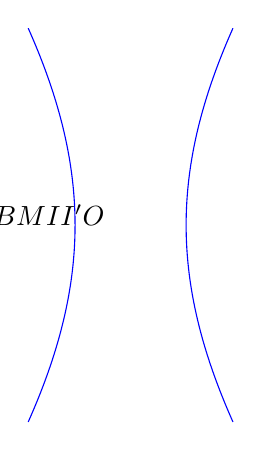
\begin{tikzpicture}[scale=1]
\tkzDefPoints{0/0/a, 2/0/o, 4/0/b, 1.3/0/m, 2.7/0/n, 2/0/o}
\tkzDefShiftPoint[o](120:2cm){c}
\tkzDefShiftPoint[o](-120:2cm){d}
\tkzDrawSegments[](a,b a,c b,c)
\draw[blue](0.7,2.5) to [bend left =24](0.7,-2.5);
\draw[blue](3.3,2.5) to [bend right =24](3.3,-2.5);
\tkzDrawPoints[size=3,fill=white](a,b,m,n,o,c)
\tkzLabelPoint[below left](a){$A$}
\tkzLabelPoint[below right](b){$B$}
\tkzLabelPoint[above right](c){$M$}
\tkzLabelPoint[below right](m){$I$}
\tkzLabelPoint[below left](n){$I'$}
\tkzLabelPoint[below ](o){$O$}
\end{tikzpicture}}
}
\end{ex} \haidong{20}

